




%%%%%%%%%%%%%%%%%%%%%%%%%%%%%%%%%%%%%%%%%%%%%%%%%%%%%%%%%%%%%%%%%
%%%%%%%%%%%%%%%%%%%%%%%%%%%%%%%%%%%%%%%%%%%%%%%%%%%%%%%%%%%%%%%%%
%%%%%%%%%%%%%%%%%%%%%%%%%%%%%%%%%%%%%%%%%%%%%%%%%%%%%%%%%%%%%%%%%

\begin{frame}[t]{Frequentist variance estimation}


Let $\varemp{\cdot}$ denote the sample variance.

\begin{block}{Calibration weighting standard errors sketch:
    \footnote{E.g.~, \textcite{deville:1993:generalizedraking,fuller:2011:sampling}.}
}

If we have $\muhatcw = \surcol{\meansur \w_i \y_i}$ and a
consistent residual estimate $\surcol{\varepsilon_i}$, then

$$
\varemp{\surcol{\w_i \varepsilon_i}} \approx \var{}{\sqrt{\Nsur} \muhatcw}.
$$

\end{block}

\only<2->{

\begin{block}{MrPlew Standard error consistency theorem sketch (Our contribution):\footnote{
This is essentially a corollary of our earlier work on the Bayesian infinitesimal jackknife.\footcite{giordano:2024:bayesij}
}}

For Bayesian hierarchical logictic regression, define
$\surcol{\varepsilon_i = \y_i - \expect{\post}{\m(\x_i^\trans \theta)}}$.
% \quad\textrm{and}\quad
% \surcol{\psi_i := \Nsur \w_i^\mrp \varepsilon_i}.

We state mild conditions under which, as $\Nsur \rightarrow \infty$,
for some $\tarcol{\mu_\infty}$ and variance $V$,
$$
\begin{aligned}
    \sqrt{\Nsur}\left(\muhatmrp - \tarcol{\mu_\infty} \right) \rightarrow{}&
    \mathcal{N}\left(0, V\right)
    \quad\textrm{ and }\\
    \varemp{ \surcol{\w_i^\mrp \varepsilon_i}}
%\surcol{\meansur (\psi_i - \overline{\psi})^2}
    \rightarrow{} V.
\end{aligned}
$$
\end{block}

\textbf{The use of $\surcol{\w_i^\mrp}$ is analogous to the use of $\surcol{\w_i}$
for frequentist variance estimation.}
}

\end{frame}

%%%%%%%%%%%%%%%%%%%%%%%%%%%%%%%%%%%%%%%%%%%%%%%%%%%%%%%%%%%%%%%%%
%%%%%%%%%%%%%%%%%%%%%%%%%%%%%%%%%%%%%%%%%%%%%%%%%%%%%%%%%%%%%%%%%
%%%%%%%%%%%%%%%%%%%%%%%%%%%%%%%%%%%%%%%%%%%%%%%%%%%%%%%%%%%%%%%%%


\begin{frame}[t]{Standard error estimation experiment}

\wholeslidefig{\BootstrapPlot{}}

%\vspace{-3em}
% It's last minute so put in the manual estimate of the time
\pause
$$
\begin{aligned}
    \textrm{Running fifty MCMC parametric bootstraps:}\quad & \approx 79 \textrm{ hours} \\
    \textrm{Computing approximate weights:}\quad &\AlexMrPawTimeSecs \textrm{ seconds}\\
\end{aligned}
$$
\end{frame}




%%%%%%%%%%%%%%%%%%%%%%%%%%%%%%%%%%%%%%%%%%%%%%%%%%%%%%%%%%%%%%%%%
%%%%%%%%%%%%%%%%%%%%%%%%%%%%%%%%%%%%%%%%%%%%%%%%%%%%%%%%%%%%%%%%%
%%%%%%%%%%%%%%%%%%%%%%%%%%%%%%%%%%%%%%%%%%%%%%%%%%%%%%%%%%%%%%%%%

\begin{frame}{Real Data: Lax Philips}
Analysis of national support for gay marriage.\footnote{Based on \textcite{kastellec:2010:laxmrp},
see also \textcite{lax:2009:gay}.}

\begin{itemize}
    %
    \item \textbf{Target population:} US Census Public Use Microdata Sample 2000
    \item \textbf{Survey population:} Combined national-level polls from 2004
    \item \textbf{Respose:}  ``Do you favor allowing gay and lesbian couples to marry legally?''
    \item For regressors, use race, gender, age, education, state, region,
        and continuous statewide religion and political characteristics, including
        some analyst--selected interactions.
    %
\end{itemize}

$$
\begin{aligned}
    \textrm{Survey observations:} &&  \surcol{\Nsur} ={}& \LaxNSur  \\
    \textrm{Target observations (rows):} &&  \tarcol{\Ntar} ={}& \LaxNTar \\
    \\
    \textrm{Uncorrected survey mean:} && \surcol{\meansur \y_i} ={}& \LaxSurmean \\
    \textrm{Raking:} && \muhat_\cal ={}& \LaxRaking \\
    \textrm{MrP:} && \muhat_\mrp ={}& \LaxMrp
        \quad(\textrm{Post. sd} = \LaxMrpSD)\\
\end{aligned}
$$
%
\end{frame}



%%%%%%%%%%%%%%%%%%%%%%%%%%%%%%%%%%%%%%%%%%%%%%%%%%%%%%%%%%%%%%%%%
%%%%%%%%%%%%%%%%%%%%%%%%%%%%%%%%%%%%%%%%%%%%%%%%%%%%%%%%%%%%%%%%%
%%%%%%%%%%%%%%%%%%%%%%%%%%%%%%%%%%%%%%%%%%%%%%%%%%%%%%%%%%%%%%%%%



\begin{frame}{Covariate balance for primary effects}
\LaxImbalancePrimary{}
\end{frame}


\begin{frame}{Covariate balance for interaction effects}
\LaxImbalanceInteraction{}
\end{frame}




\begin{frame}[t]{Predictions}
    \LaxPredictionFigOne{}
\end{frame}


\begin{frame}[t]{Predictions and actual MCMC results}
    \LaxPredictionFigTwo{}
    \vspace{-3em}
    $$
    \begin{aligned}
        \textrm{Running ten MCMC refits:}\quad & \LaxRefitTimeHours \textrm{ hours} &
        \textrm{Computing approximate weights:}\quad &\LaxMrPawTimeSecs \textrm{ seconds}\\
    \end{aligned}
    $$
\end{frame}



%%%%%%%%%%%%%%%%%%%%%%%%%%%%%%%%%%%%%%%%%%%%%%%%%%%%%%%%%%%%%%%%%
%%%%%%%%%%%%%%%%%%%%%%%%%%%%%%%%%%%%%%%%%%%%%%%%%%%%%%%%%%%%%%%%%
%%%%%%%%%%%%%%%%%%%%%%%%%%%%%%%%%%%%%%%%%%%%%%%%%%%%%%%%%%%%%%%%%




\def\res{\varepsilon}
\def\w{w}
\def\wtil{\tilde{\w}}
\def\reshat{\hat{\res}}

\def\methodrow#1#2#3{
\begin{minipage}[t]{0.15\textwidth}
    \centering
    %\rotatebox{90}{#1}
    #1
\end{minipage}
\hfill
\begin{minipage}[t]{0.4\textwidth}
    \centering
    \vspace{-2em}
    #2
    \pause
\end{minipage}
\hfill
\begin{minipage}[t]{0.4\textwidth}
    \centering
    \vspace{-2em}
    #3
    \pause
\end{minipage}
}


\def\methodspacer{
    \vspace{1em}
    \hrule
    \vspace{1em}
}

\begin{frame}{Some generalized diagnostics}

\vspace{2em}
\methodrow{\,}{\textbf{Regression}}{\textbf{General models}}

\methodrow{Consistency /\\ Unbiased}
{
$$
\begin{aligned}
    \y ={}& \theta^\trans \x + \res \\
    \ytil ={}& (\theta + \delta)^\trans \x + \res \\
    \thetahat(\ytil) \eqcheck{}& \thetahat(\y) + \delta
\end{aligned}
$$
}{
$$
\begin{aligned}
    \y ={}& \f(\x, \varepsilon, \theta) \\
    \ytil ={}& \f(\x, \varepsilon, \theta + \delta) \\
    \thetahat(\ytil) \eqcheck{}& \thetahat(\y) + \delta
\end{aligned}
$$
}

\methodspacer

\methodrow{Exogonous\\residuals}
{
$$
\begin{aligned}
    \y ={}& \theta^\trans \x + \res \\
    \ytil ={}& \y + \res \z \\
    \thetahat(\ytil) \eqcheck{}& \thetahat(\y)
\end{aligned}
$$
}{
$$
\begin{aligned}
    \y \sim{}& \p(\y \vert \x) \textrm{ and } \p(\x) ={} \w \\
    \wtil ={}& \w + \delta z \\
    \thetahat(\wtil) \eqcheck{}& \thetahat(\w)
\end{aligned}
$$
}


\methodspacer


\methodrow{Fisher information}
{
$$
\begin{aligned}
    %\y ={}& \theta^\trans \x + \res \\
    \mathcal{I} :={}& \textrm{Fisher information}\\
    \Sigma :={}& \textrm{Score covariance} \\
    \mathcal{I}^{-1} \eqcheck{}& \Sigma
\end{aligned}
$$
}{
$$
\begin{aligned}
    \y \sim{}& \p(\y \vert \theta) \\
    \ytil \sim{}& \textrm{Importance sample }\y\\
    &\textrm{ using }\wtil ={} \frac{\p(\y \vert \thetahat + \delta)}{\p(\y \vert \thetahat)} \\
    \thetahat(\wtil) \eqcheck{}& \thetahat(1) + \delta
\end{aligned}
$$
}


\vspace{2em}


\end{frame}



%%%%%%%%%%%%%%%%%%%%%%%%%%%%%%%%%%%%%%%%
%%%%%%%%%%%%%%%%%%%%%%%%%%%%%%%%%%%%%%%%
%%%%%%%%%%%%%%%%%%%%%%%%%%%%%%%%%%%%%%%%

\begin{frame}{Weights by education for the Name Change analysis}

    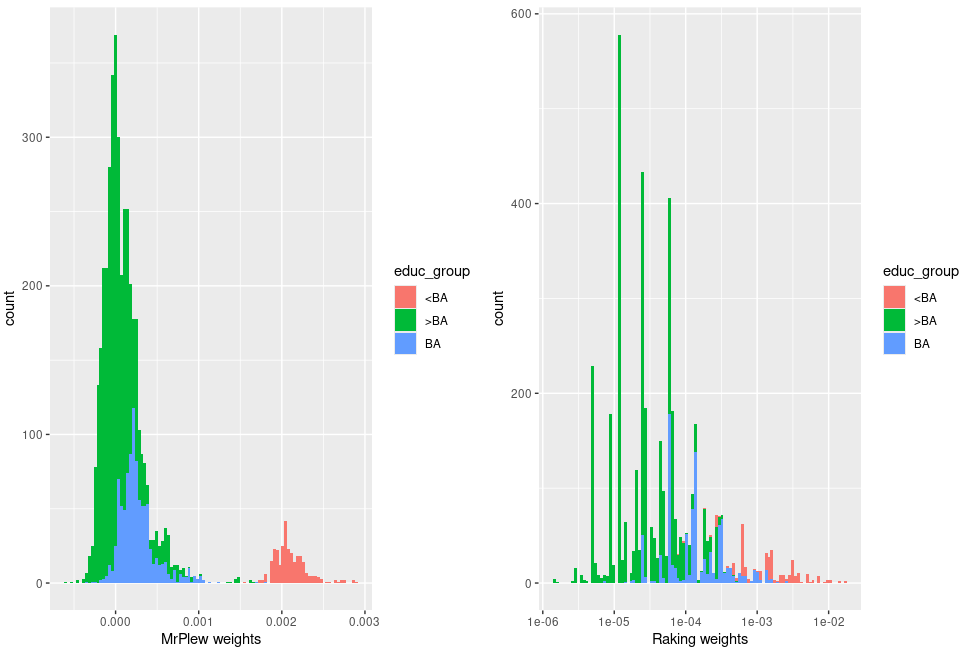
\includegraphics[width=0.8\textwidth]{static_figures/w_educ_hist.png}
\end{frame}



%%%%%%%%%%%%%%%%%%%%%%%%%%%%%%%%%%%%%%%%
%%%%%%%%%%%%%%%%%%%%%%%%%%%%%%%%%%%%%%%%
%%%%%%%%%%%%%%%%%%%%%%%%%%%%%%%%%%%%%%%%


